\documentclass[a4paper]{jpconf}
\usepackage{amsmath}
\usepackage{amssymb}
\usepackage[UKenglish]{babel}
\usepackage{graphicx}
\usepackage{hyperref}
\hypersetup{colorlinks=false, bookmarks=true}
\usepackage{float}
\usepackage{comment}
\usepackage{caption}
\usepackage[skip=0.5ex]{subcaption}
\usepackage{xcolor}

\hyphenation{few-femto-second}

\begin{document}
%\maketitle

\twocolumn[

\pagenumbering{arabic}
\title{Modelling of nonlinear light up-conversion from intense femtosecond laser pulses}
\author{David Amorim (University of Glasgow)}
\address{DESY Summer Student Programme 2023 \\ Group:  Attosecond Science (CFEL-ATTO) \\ Institute: Centre for Free-Electron Laser Science (CFEL)\\ Supervisor: Josina Hahne}

\begin{abstract}
\textcolor{red}{XXXX}
\end{abstract}
]


\thispagestyle{plain}
\pagestyle{plain}
\setlength{\footskip}{20pt}

\section{Introduction}
The electronic motion associated with chemical reactions and atomic energy transitions takes place on femotsecond ($1 \text{fs} = 10^{-15} \text{s}$) to attosecond ($1 \text{as} = 10^{-18} \text{s}$) time scales. Time-resolved imaging of molecular dynamics therefore requires ultrashort laser pulses in the few-femtosecond regime. An important type of electronic motion is that excited by the absorption of ultraviolet (UV) radiation: a variety of biochemical processes, such as DNA damage, are known to be caused by UV excitation. Generating few-femtosecond UV pulses for time-resolved measurements of UV-excited molecules plays a crucial part in further understanding and eventually controlling these effects. \par 
The CFEL-ATTO group at DESY produces ultrashort UV pulses in the femtosecond regime via third-harmonic generation (THG) in a gas cell \cite{galli2019}. This process is sensitive to a large range of parameters which affect the duration and energy of the generated UV pulse. Numerical simulations of the interactions between the laser pulse and the gas can therefore be advantageous to better understand how THG takes place and how it is affected by the experimental conditions. \par 
This report summarises the work carried out as part of a DESY Summer Student project focussed on producing simulations of the THG process. The simulations were mainly carried out using the propagation solver \textit{Luna.jl} (\cite{brahms2023}) while the \textit{COMSOL Multiphysics} software was used to model the gas density distribution. The aim of the simulations was to reproduce the experimental conditions in the gas, in order to study which effects dominate the THG process and the shaping of the UV pulse. Further, parameter scans were simulated to investigate how changes to different variables in the experimental set-up affect the output pulse. \par 
\textcolor{red}{
briefly list findings (main relevant processes in gas, experimental conditions...)
}

\section{Theoretical Background}
This section gives a brief overview of key properties of ultrashort (femtosecond) laser pulses,  THG and other relevant nonlinear optical effects, as well as the differential equation describing the propagation of ultrafast laser pulses. An in-depth treatment of these topics can be found in textbooks like \cite{keller2021, new2011}. 

\subsection{Ultrashort Laser Pulses}
An ultrashort laser pulse can be described as a carrier wave at carrier frequency $\omega_0$ with an amplitude modulated by an envelope function. In the femtosecond domain the envelope may only contain a few cycles of the carrier wave. Using the analytic representation of the electric field vector the time-domain representation of an ultrashort laser pulse can be written as 
\begin{equation}
\mathbf{E}(t, \mathbf{r}) = \mathbf{A}(t, \mathbf{r}) e^{i[ \omega_o t + \phi(t)]},
\end{equation}
where $\mathbf{A}(t, \mathbf{r})$ represents the envelope function and $\phi(t)$ is the temporal phase. The vectorial nature of the envelope takes into account the polarisation of the pulse. Similarly, the frequency-domain representation is 
\begin{equation}
\mathbf{E}(\omega, \mathbf{r}) = \mathbf{A}'(\omega, \mathbf{r}) e^{i \varphi(\omega)},
\end{equation}
where $\varphi(\omega)$ is the spectral phase. Note that the effect of the carrier term in the frequency domain is merely a shift along the frequency axis and can be thus be absorbed in the definition of $\omega$. \par 
The spectral and temporal phase are commonly expanded as Taylor-series, with the notation $\phi_n \equiv \frac{\partial^n \phi}{\partial t^n}$ and $\varphi_n \equiv \frac{\partial^n \varphi}{\partial \omega^n}$ used to denote the series coefficients. The zeroth-order terms of both expansions are the same, $\phi_0 = \varphi_0$, and correspond to the carrier-envelope phase (CEP), also known as the absolute phase. The CEP desribes the phase difference between the carrier and the envelope and is particularly relevant for few-cycle pulses. A laser pulse with no terms in $\varphi(\omega)$ higher than $\varphi_0$ is said to be transform-limited. A pulse is said to be chirped if there are nonlinear terms in $\phi(t)$ or $\varphi(\omega)$. \par 
The presence of chirp can result in both spectral and temporal broadening of the pulse envelope. A convenient measure of chirp is therefore the so-called time-bandwidth product $\Delta \omega \Delta t$, where $\Delta \omega$ is the full-width half-maximum (FWHM) of $\mathbf{A}'(\omega, \mathbf{r})$ and $\Delta t$ the FWHM of $\mathbf{A}(t, \mathbf{r})$. It can be shown that the time-bandwidth product is minimised for transform-limited, i.e. unchirped, pulses. In other words, at a given spectral bandwidth the shortest pulse durations are associated with transform-limited pulses, for which case the relation $\Delta \omega \propto (\Delta t)^{-1}$ holds. \par 
The effects on a laser pulse when travelling through a medium can be described via additional terms in the spectral phase: $\varphi(\omega) \to \varphi(\omega) + [\beta(\omega) + i \alpha(\omega)]L$, where $L$ corresponds to the distance travelled in a medium, $\beta(\omega)$ is the propagation coefficient, and $\alpha(\omega)$ the absorption coefficient. The latter term represents an attenuation of the pulse while the former has the effect of introducing chirp (provided the Taylor-expansion of $\beta(\omega)$ has non-zero terms higher than $\beta_1$). Note that depending on the signs of the quantities involved, the chirp due to $\beta(\omega)$ will either increase or compensate the existing chirp on the pulse. Thus, an initially positively chirped pulse will further broaden upon propagation through a normally dispersive medium while a negatively chirped pulse will be compressed. The opposite effect is observed in anomalously dispersive media.

\subsection{Nonlinear Optics and THG}
For most materials, the polarisation response to an electric field of moderate intensity is linear. The peak intensities reached in ultrashort laser pulses are large enough, however, for this approximation to become invalid and nonlinear polarisation components to appear. The resulting polarisation can then be represented as a combination of a linear and a nonlinear term: $\mathbf{P}(t, \mathbf{r}) = \mathbf{P}^\text{L}(t, \mathbf{r}) + \mathbf{P}^\text{NL}(t, \mathbf{r})$, where spatial dependencies have been left implicit. \par 
The linear polarisation is given by the familiar expression $\mathbf{P}^\text{L}(t, \mathbf{r}) = \epsilon_0 \chi_e \mathbf{E}(t, \mathbf{r})$, where $\chi_e$ is the (linear) electric susceptibility. The nonlinear term, $\mathbf{P}^\text{NL}(t, \mathbf{r})$, on the other hand, is less trivial. It can be approximated using a perturbative approach in combination with a term that takes into account the effects of photoionisation, which is non-perturbative:
\begin{equation}\label{eq:p_nl}
\mathbf{P}^\text{NL}(t, \mathbf{r}) = \epsilon_0 \sum_{n=2} \chi^{(n)} [\mathbf{E}(t, \mathbf{r})]^n + \mathbf{P}^\text{ion}(t, \mathbf{r}),
\end{equation}
where $\chi^{(n)}$ is the $n$-th order electric susceptibility. Note that for gases the assumption that the higher-order susceptibilities are frequency-independent scalars is a good approximation. Further note that the series expansion starts at the quadratic term as the linear term is contained in $\mathbf{P}^\text{L}(t, \mathbf{r})$.  \par 
In centrosymmetric media such as gases all even-order susceptibilities necessarily vanish, so that the dominant term in the expansion is the third-order term. Higher-order contributions can be neglected to a good approximation, so that \eqref{eq:p_nl} becomes 
\begin{equation}\label{eq:p_nl_simpl}
\mathbf{P}^\text{NL}(t, \mathbf{r}) = \epsilon_0 \chi^{(3)} [\mathbf{E}(t, \mathbf{r})]^3 + \mathbf{P}^\text{ion}(t, \mathbf{r}),
\end{equation}
where $[\mathbf{E}(t, \mathbf{r})]^3 \equiv \mathbf{E}(t, \mathbf{r}) |\mathbf{E}(t, \mathbf{r})|^2$. 
The first term in \eqref{eq:p_nl_simpl} is known as the Kerr term and its presence leads directly to THG. This can be seen when considering an oscillating electric field $\mathbf{E}(t, \mathbf{r}) = \hat{\mathbf{E}}(t, \mathbf{r})\cos(\omega t)$. The resulting Kerr response then is 
\begin{align}\label{eq:Kerr_response}
\nonumber  \mathbf{P}^\text{Kerr}(t,\mathbf{r}) &= \epsilon_0 \chi^{(3)} [\hat{\mathbf{E}}(t, \mathbf{r})]^3 \cos^3(\omega t) \\ &= \frac{\epsilon_0}{4}  \chi^{(3)} [\hat{\mathbf{E}}(t, \mathbf{r})]^3 \left\{ \cos (3\omega t) +  3 \cos(\omega t)\right\}.
\end{align}
The first summand in \eqref{eq:Kerr_response} corresponds to a field contribution oscillating at the frequency $3 \omega$. Thus, a pump wave at the fundamental frequency $\omega$ will generate a co-propagating frequency-tripled field. This process can be identified as THG. Note that THG is just once instance of a range of nonlinear optical effects which result in the generation of higher-frequency waves from a driving field, generally known as frequency up-conversion. \par 
The intensity of the third harmonic, and by extension the THG efficiency $\eta_{THG}$, is determined by the value of $\chi^{(3)}$ in a given medium as well as the d by the intensity of the driving field. This also implies that, since the intensity of the fundamental pulse is highest at the peak of the envelope, THG conversion is more efficient there so that the third harmonic pulse is narrower in time than the input pulse by a factor of $\sim\sqrt{3}$. \par 
 A further factor to consider is that the third harmonic is generated in-phase with the driving wave at each point in the nonlinear medium. Thus, in dispersive media there will be phase differences between third harmonic contributions generated at different points along the crystal. This can result in destructive interference and thus lower the THG conversion efficiency. \par 
The second summand in \eqref{eq:Kerr_response}, corresponding to polarisation response at the fundamental frequency, is also significant: its effect is a correction term in the refractive index that is proportional to the intensity of the driving field. This intensity-dependent refractive index (IDRI) produced by the Kerr term has important implications for the propagation of laser pulses in nonlinear media. These include self-phase modulation (SPM) as well as self-steepening. SPM arises because the intensity of a laser pulse is higher at the peak of its envelope than at the wings, so that the peak will experience a higher refractive index, and therefore phase shift on propagation, than the edges of the pulse. This induces chirp and can result in spectral broadening. Similarly, self-steepening describes the effect of the peak of the pulse experiencing, due to the IDRI, a different group velocity in a dispersive medium than the wings. This results in the leading edge of the pulse or, in the case of anomalous dispersion, the trailing edge, to get steeper on propagation, corresponding to temporal compression and spectral broadening. \par 
After having considered the effects of the Kerr term in the previous paragraphs, we now turn to the second term in \eqref{eq:p_nl}: the nonlinear polarisation due to photoionisation. The highly energetic driving pulse can ionise the atoms or molecules in the nonlinear medium, resulting in the presence of free electrons. This has a two-fold effect on pulse propagation and THG. On the one hand, the pump field is depleted since it must overcome the atomic ionisation potential, so that less energy is available to drive THG. On the other hand, the freed electrons also interact electromagnetically with the fundamental and third harmonic fields, which results in spatio-temporal reshaping of the pulses. Thus, despite ionisation limiting the achievable third harmonic pulse energy, it can aid in further shortening the generated pulses. \par 
The theoretical treatment of $\mathbf{P}^\text{ion}(t, \mathbf{r})$ is significantly more sophisticated than that of the Kerr term. As is derived in \cite{geissler1999}:
\begin{equation}\label{eq:p_ion}
\frac{\partial}{\partial t} \mathbf{P}^\text{ion}(t, \mathbf{r}) = \frac{I_p}{\mathbf{E}(t)} \frac{\partial n_e}{\partial t} + \frac{e^2}{m_e^2} \int_{-\infty}^t n_e(t') \mathbf{E}(t')dt',
\end{equation} 
where $n_e(t)$ is the number of free electrons at any point in time, $I_p$ is the ionisation potential, and $e$, $m_e$ represent the electron charge and mass, respectively. The value of $n_e(t)$ can be found from 
\begin{equation}
\frac{\partial n_e}{\partial t} = (n_e - n_0) W(\mathbf{E}),
\end{equation}
where $n_0$ is the initial number of neutral atoms and $W(\mathbf{E})$ is the ionisation rate, which can be calculated from the so-called ADK model of tunnel ionisation or the PPT model, which is more sophisticated but also more computationally expensive. 

\subsection{The Unidirectional Pulse Propagation Equation}

A variety of different differential equations  can be used to describe the propagation of laser pulses. Many of them are derived under the slowly-varying- envelope assumption (SVEA), which approximates the carrier wave to change significantly more quickly in space and time than the pulse envelope. The SVEA does not hold for ultrashort pulses, however, and hence many commonly used pulse propagation equations are not suitable for the study of few-femtosecond pulses. The unidirectional pulse propagation equation (UPPE) is derived directly from Maxwell's equations without additional approximations, see \cite{kolesik2004}, and therefore can be applied to ultrashort pulses. It is the differential equation used by \textit{Luna.jl} to simulate laser pulse propagation. This section gives a brief overview of the UPPE and how it is solved in \textit{Luna.jl}. For more details on numerical solutions of the UPPE see the \textit{Luna.jl} documentation, \cite{brahms2023}, as well as \cite{tani2014}. \par 
The general form of the UPPE for a laser pulse of frequency $\omega$ travelling in the $z$-direction is
\begin{align}\label{eq:UPPE}
\nonumber \frac{\partial}{\partial z} \mathbf{E}(\omega, \mathbf{k}_\perp, z)&= \mathcal{L}(\omega, z)\mathbf{E}(\omega, \mathbf{k}_\perp, z) \\ &+ \frac{i \omega}{N} \mathbf{P}^\text{NL}(\omega, \mathbf{k}_\perp, z),
\end{align}
where $\mathbf{E}(\omega, \mathbf{k}_\perp, z)$ is the reciprocal-space electric field amplitude in the frequency domain, $\mathbf{k}_\perp$ is the transverse spatial frequency vector,  $\mathcal{L}(\omega, z)$ is a linear operator describing dispersion and absorption, $\mathbf{P}^\text{NL}(\omega, \mathbf{k}_\perp, z)$ is the frequency-domain nonlinear polarisation in reciprocal space and $N$ is a normalisation factor. \par 
For a laser pulse propagating in a gas, not confined by a fibre or waveguide, the linear operator $\mathcal{L}(\omega, z)$ is given by 
\begin{equation}\label{eq:Lj}
\mathcal{L}(\omega, z) = i \left( \beta(\omega, z) - \frac{\omega}{v} \right) - \frac{1}{2} \alpha (\omega,z),
\end{equation}
where $\beta(\omega,z)$ is the propagation coefficient of the gas, $v$ is a reference frame velocity (chosen to be the group velocity at the central wavelength $\lambda_0$), and $\alpha(\omega,z)$ is the absorption coefficient of the gas. \par 



As is seen in \eqref{eq:p_nl_simpl} and \eqref{eq:p_ion}, the nonlinear polarisation is naturally calculated from the electric field in real space and the time domain. Thus, numerically solving the UPPE, which lives in reciprocal space and the frequency domain, requires a cycle of temporal Fourier transforms into and out of the frequency domain as well as transverse spatial transforms into and out reciprocal space at each step. The choice of transverse spatial transform is determined by the geometry of the system. \par 
Since the beam and the gas channel it propagates through for UV generation are approximately radially symmetric, a zeroth-order Hankel transform is chosen as the transverse spatial transform. This is mathematically equivalent to a  transverse spatial Fourier transform in Cartesian coordinates but is computationally more efficient, as the Hankel transform exploits the symmetry and only involves integration in the radial direction, whereas the transverse spatial Fourier transform is two-dimensional. 
 
\section{Experimental Conditions}
This section summarises the experimental conditions which were the basis of the simulations. \par 
The CFEL-ATTO group generates few-femtosecond UV laser pulses via THG in a gas cell. This is driven by a pulsed near-infrared (NIR) Ti:sapphire laser with a central wavelength of 750nm and a repetition rate of 1kHz. Various fibre-based pulse-shaping and compression techniques are used to produce NIR pulses with a duration of 5-6fs and a pulse energy of up to 3mJ. A (variable) fraction of the pump beam is then linearly polarised and focussed into a vacuum chamber for UV generation, resulting in a spatially approximately Gaussian beam with a beam waist of 65$\mu$m at the focus. The chamber contains a fused silica (SiO$_2$) chip, a gas nozzle and a pumping system. Its specifications are central to the THG process and are described in more detail in the following. \par 
The fused silica chip is equipped with a laser machined central 3mm-long channel with a 0.5mm diameter. Pressurised gas is pumped through the channel, with a two-stage differential pumping system on both sides of the central cell ensuring a tight confinement of the gas in this region. As the pump beam passes through the cell and interacts with the pressurised gas, THG takes place which results in UV pulses being generated. The UV components are then separated from the pump beam upon exiting the vacuum chamber using dispersive mirrors, which reflect in the UV but transmit in the NIR. 
\textcolor{red}{INCLUDE FIGURE? MENTION OLD/NEW CHIPS?}

\section{Simulation Results}

\textcolor{red}{section 1: comparison with experiment; section 2: investigate additional parameters; section 3: gas cell}

\textcolor{red}{test image}
\begin{center}
\begin{figure}
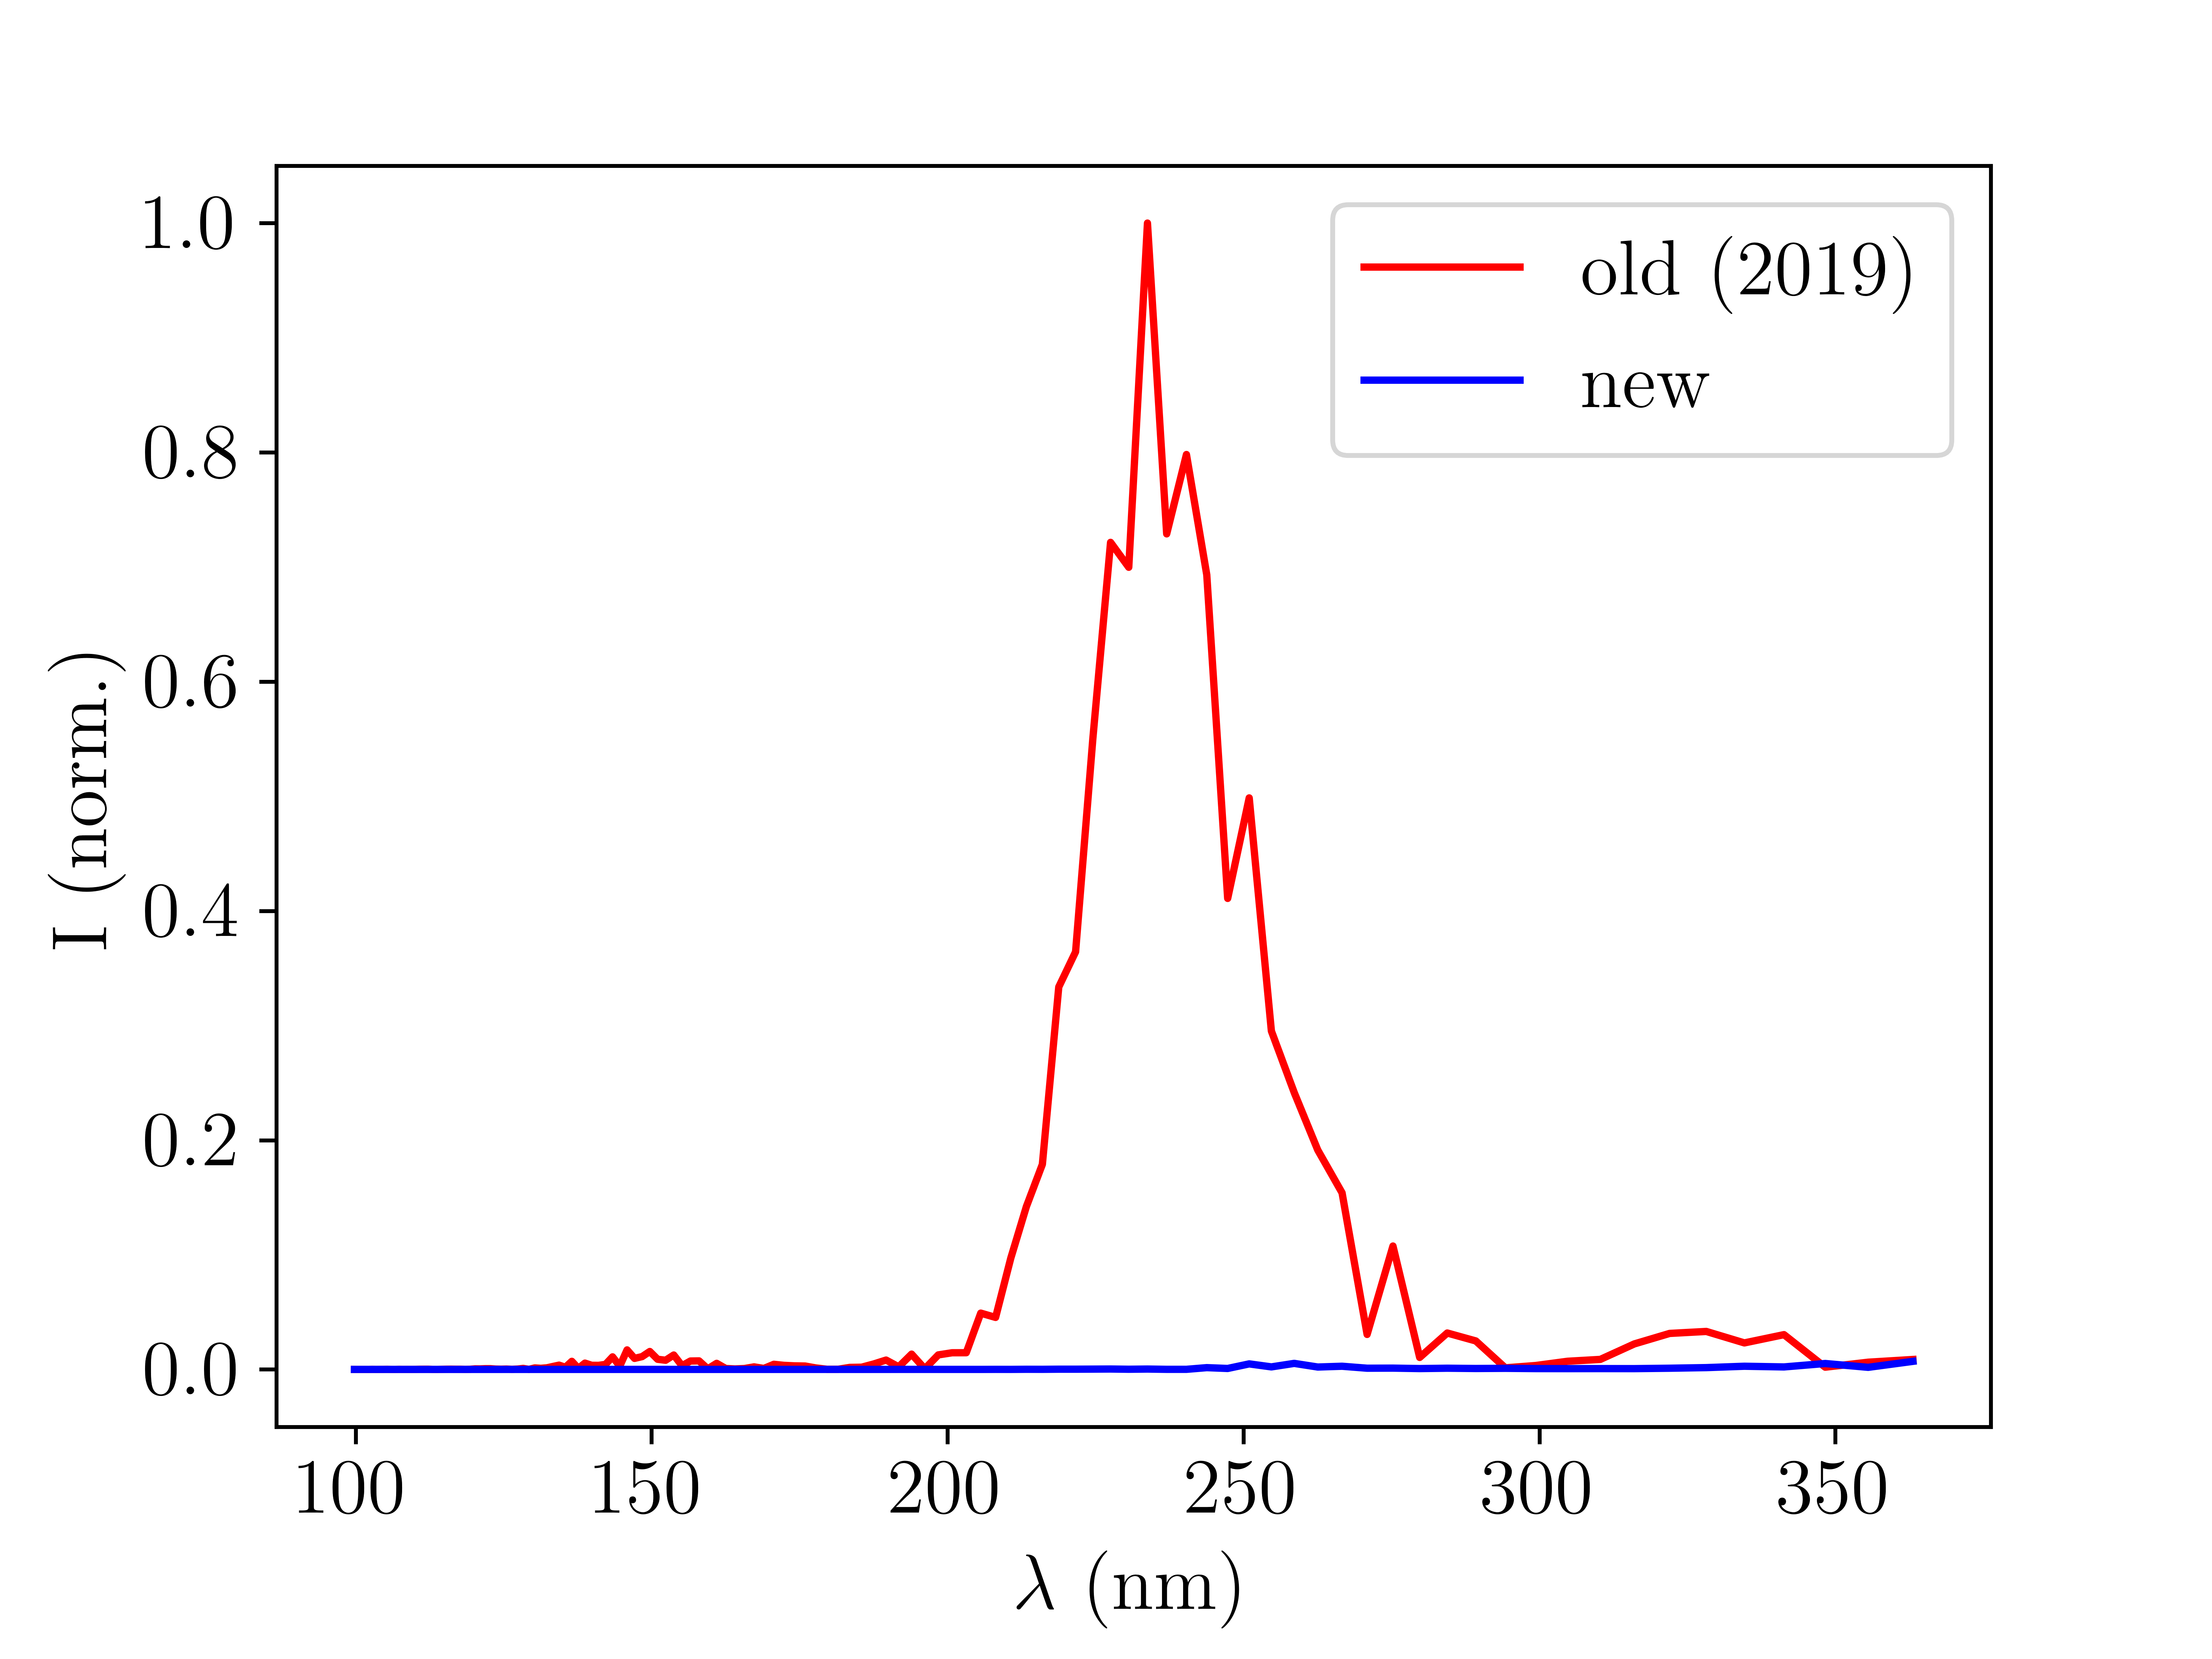
\includegraphics[scale=0.5]{im/Ar_prelim_sim_v_measured}\label{im:sim_v_measured}
\caption{Measured and simulated UV output spectrum of Argon at 150mW input beam power and 0.4bar central pressure.}
\end{figure}
\end{center}

\textcolor{red}{test image}
\begin{center}
\begin{figure}
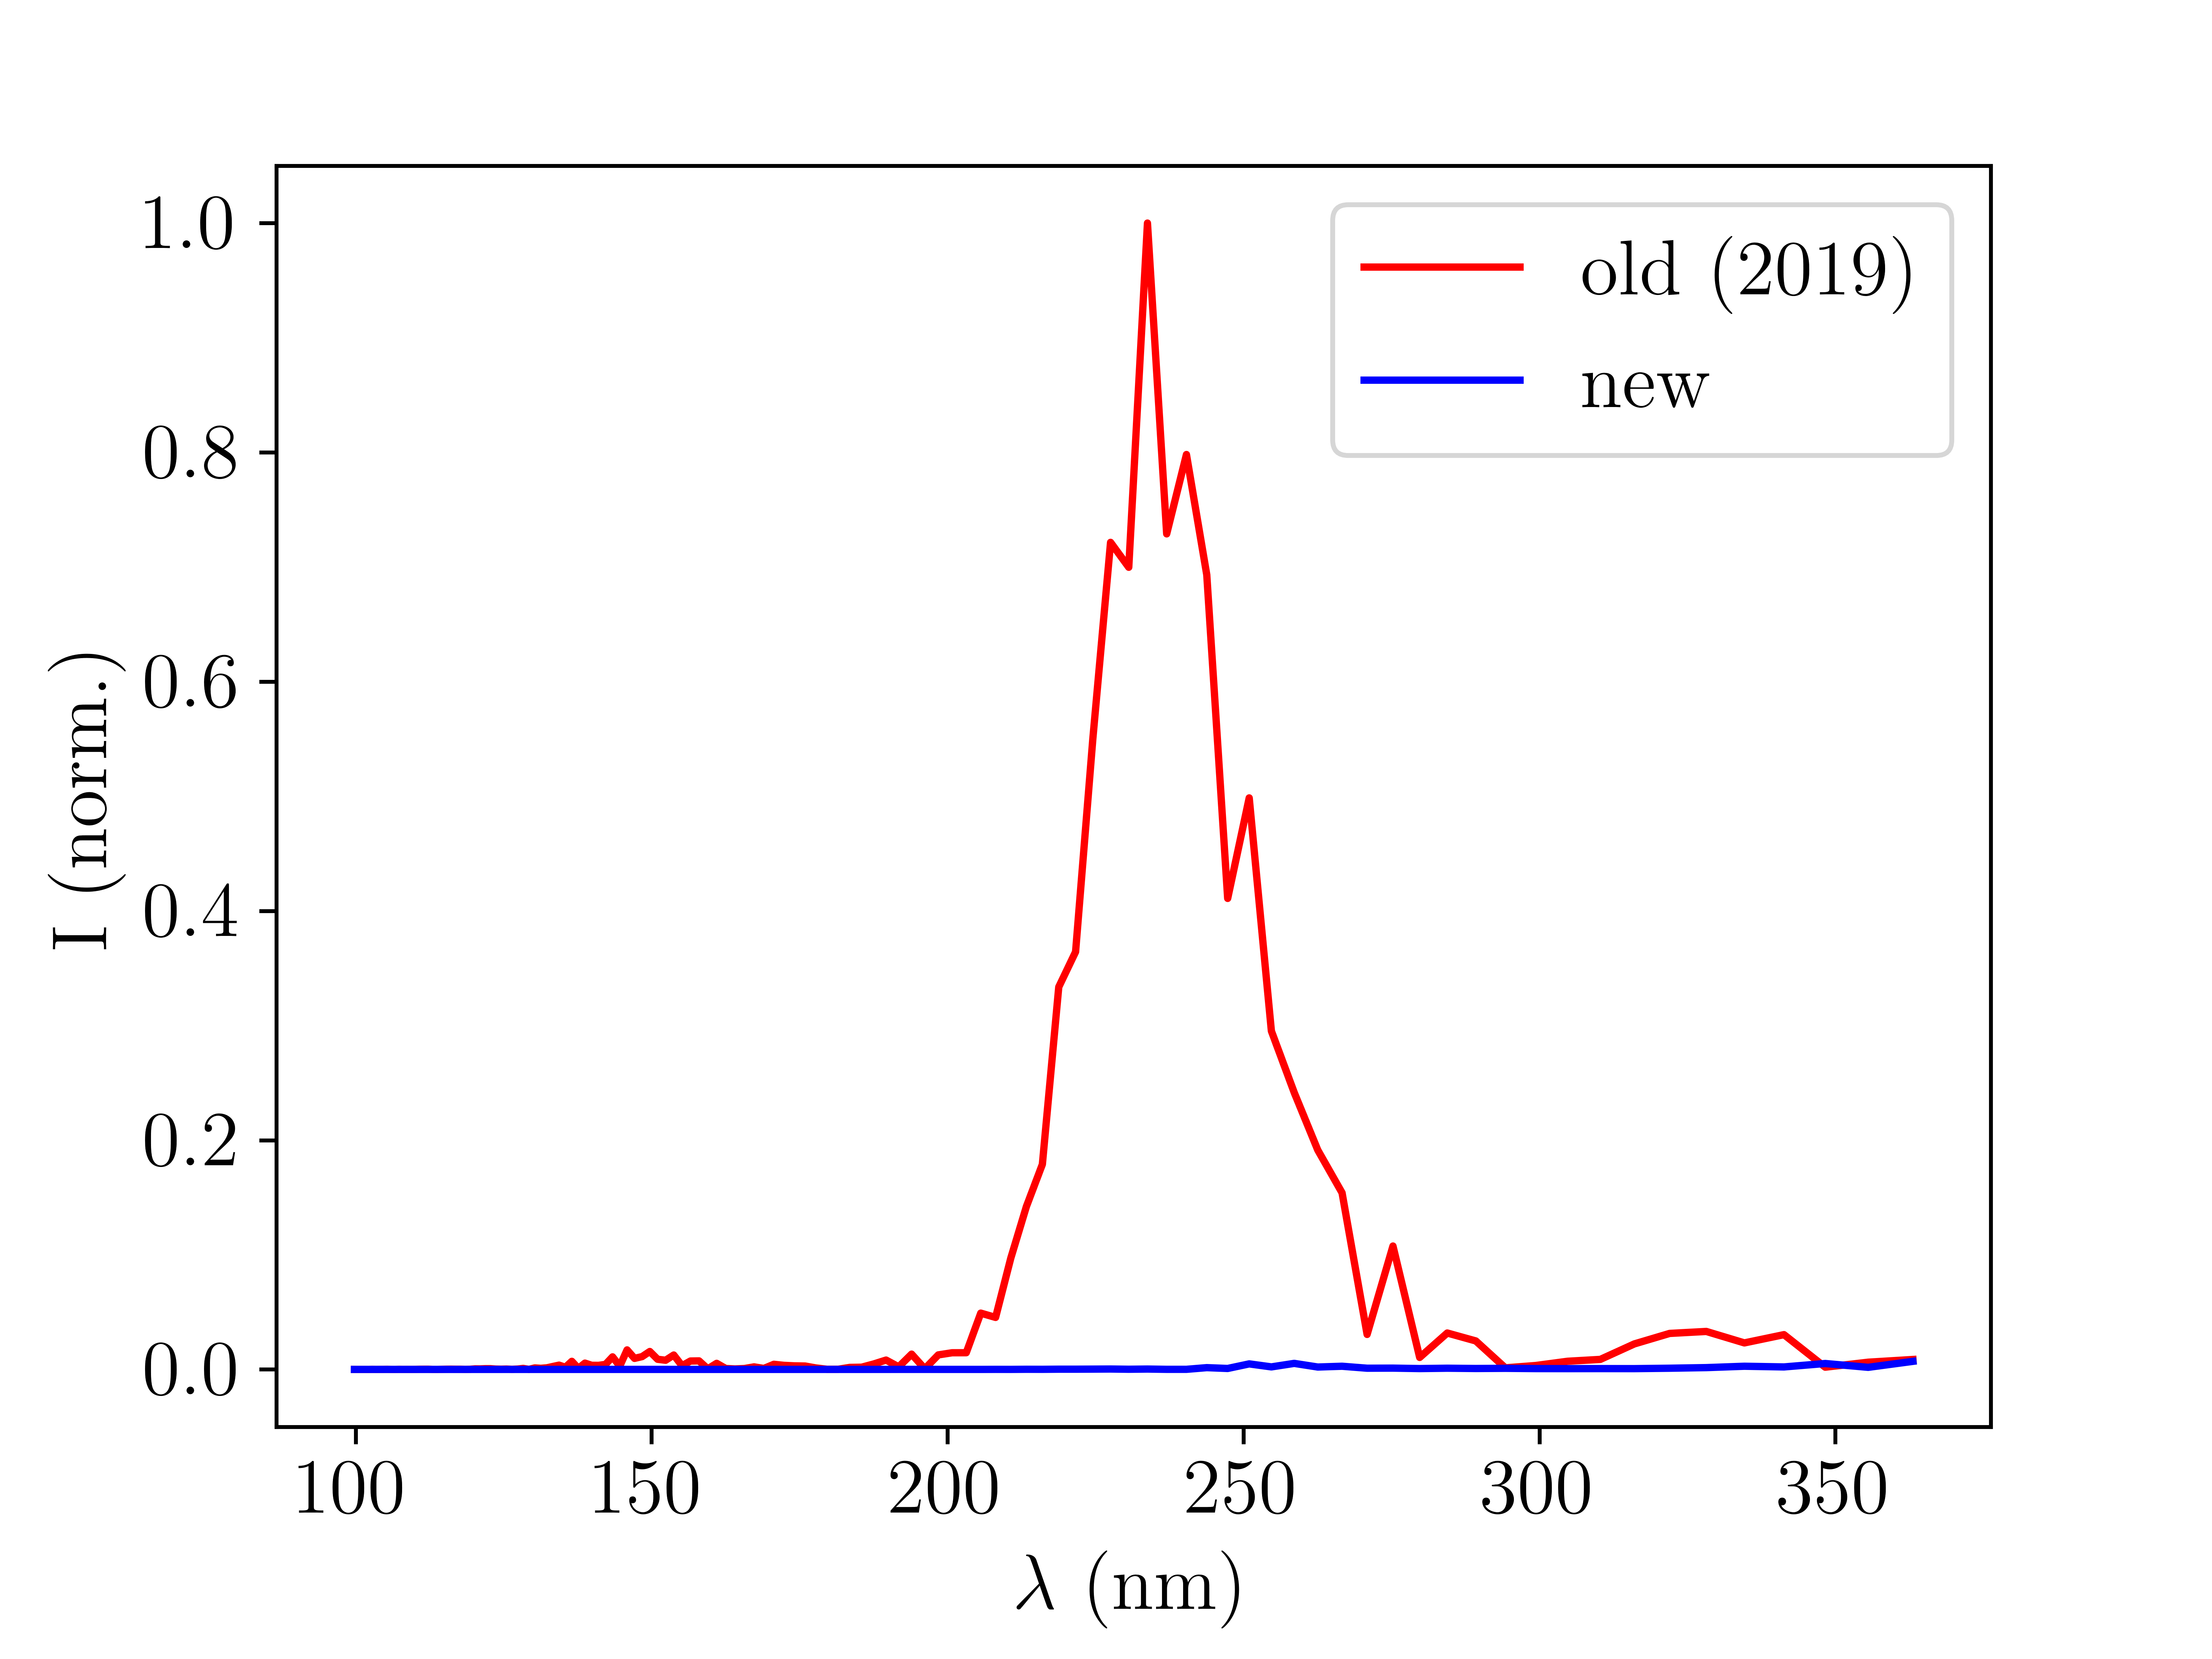
\includegraphics[scale=0.5]{im/Ar_prelim_old_vs_new}\label{im:old_v_new}
\caption{Simulated UV output spectrum of Argon at 150mW input beam power and 0.4bar central pressure with old and new gas cell design.}
\end{figure}
\end{center}

\textcolor{red}{test image}
\begin{center}
\begin{figure}
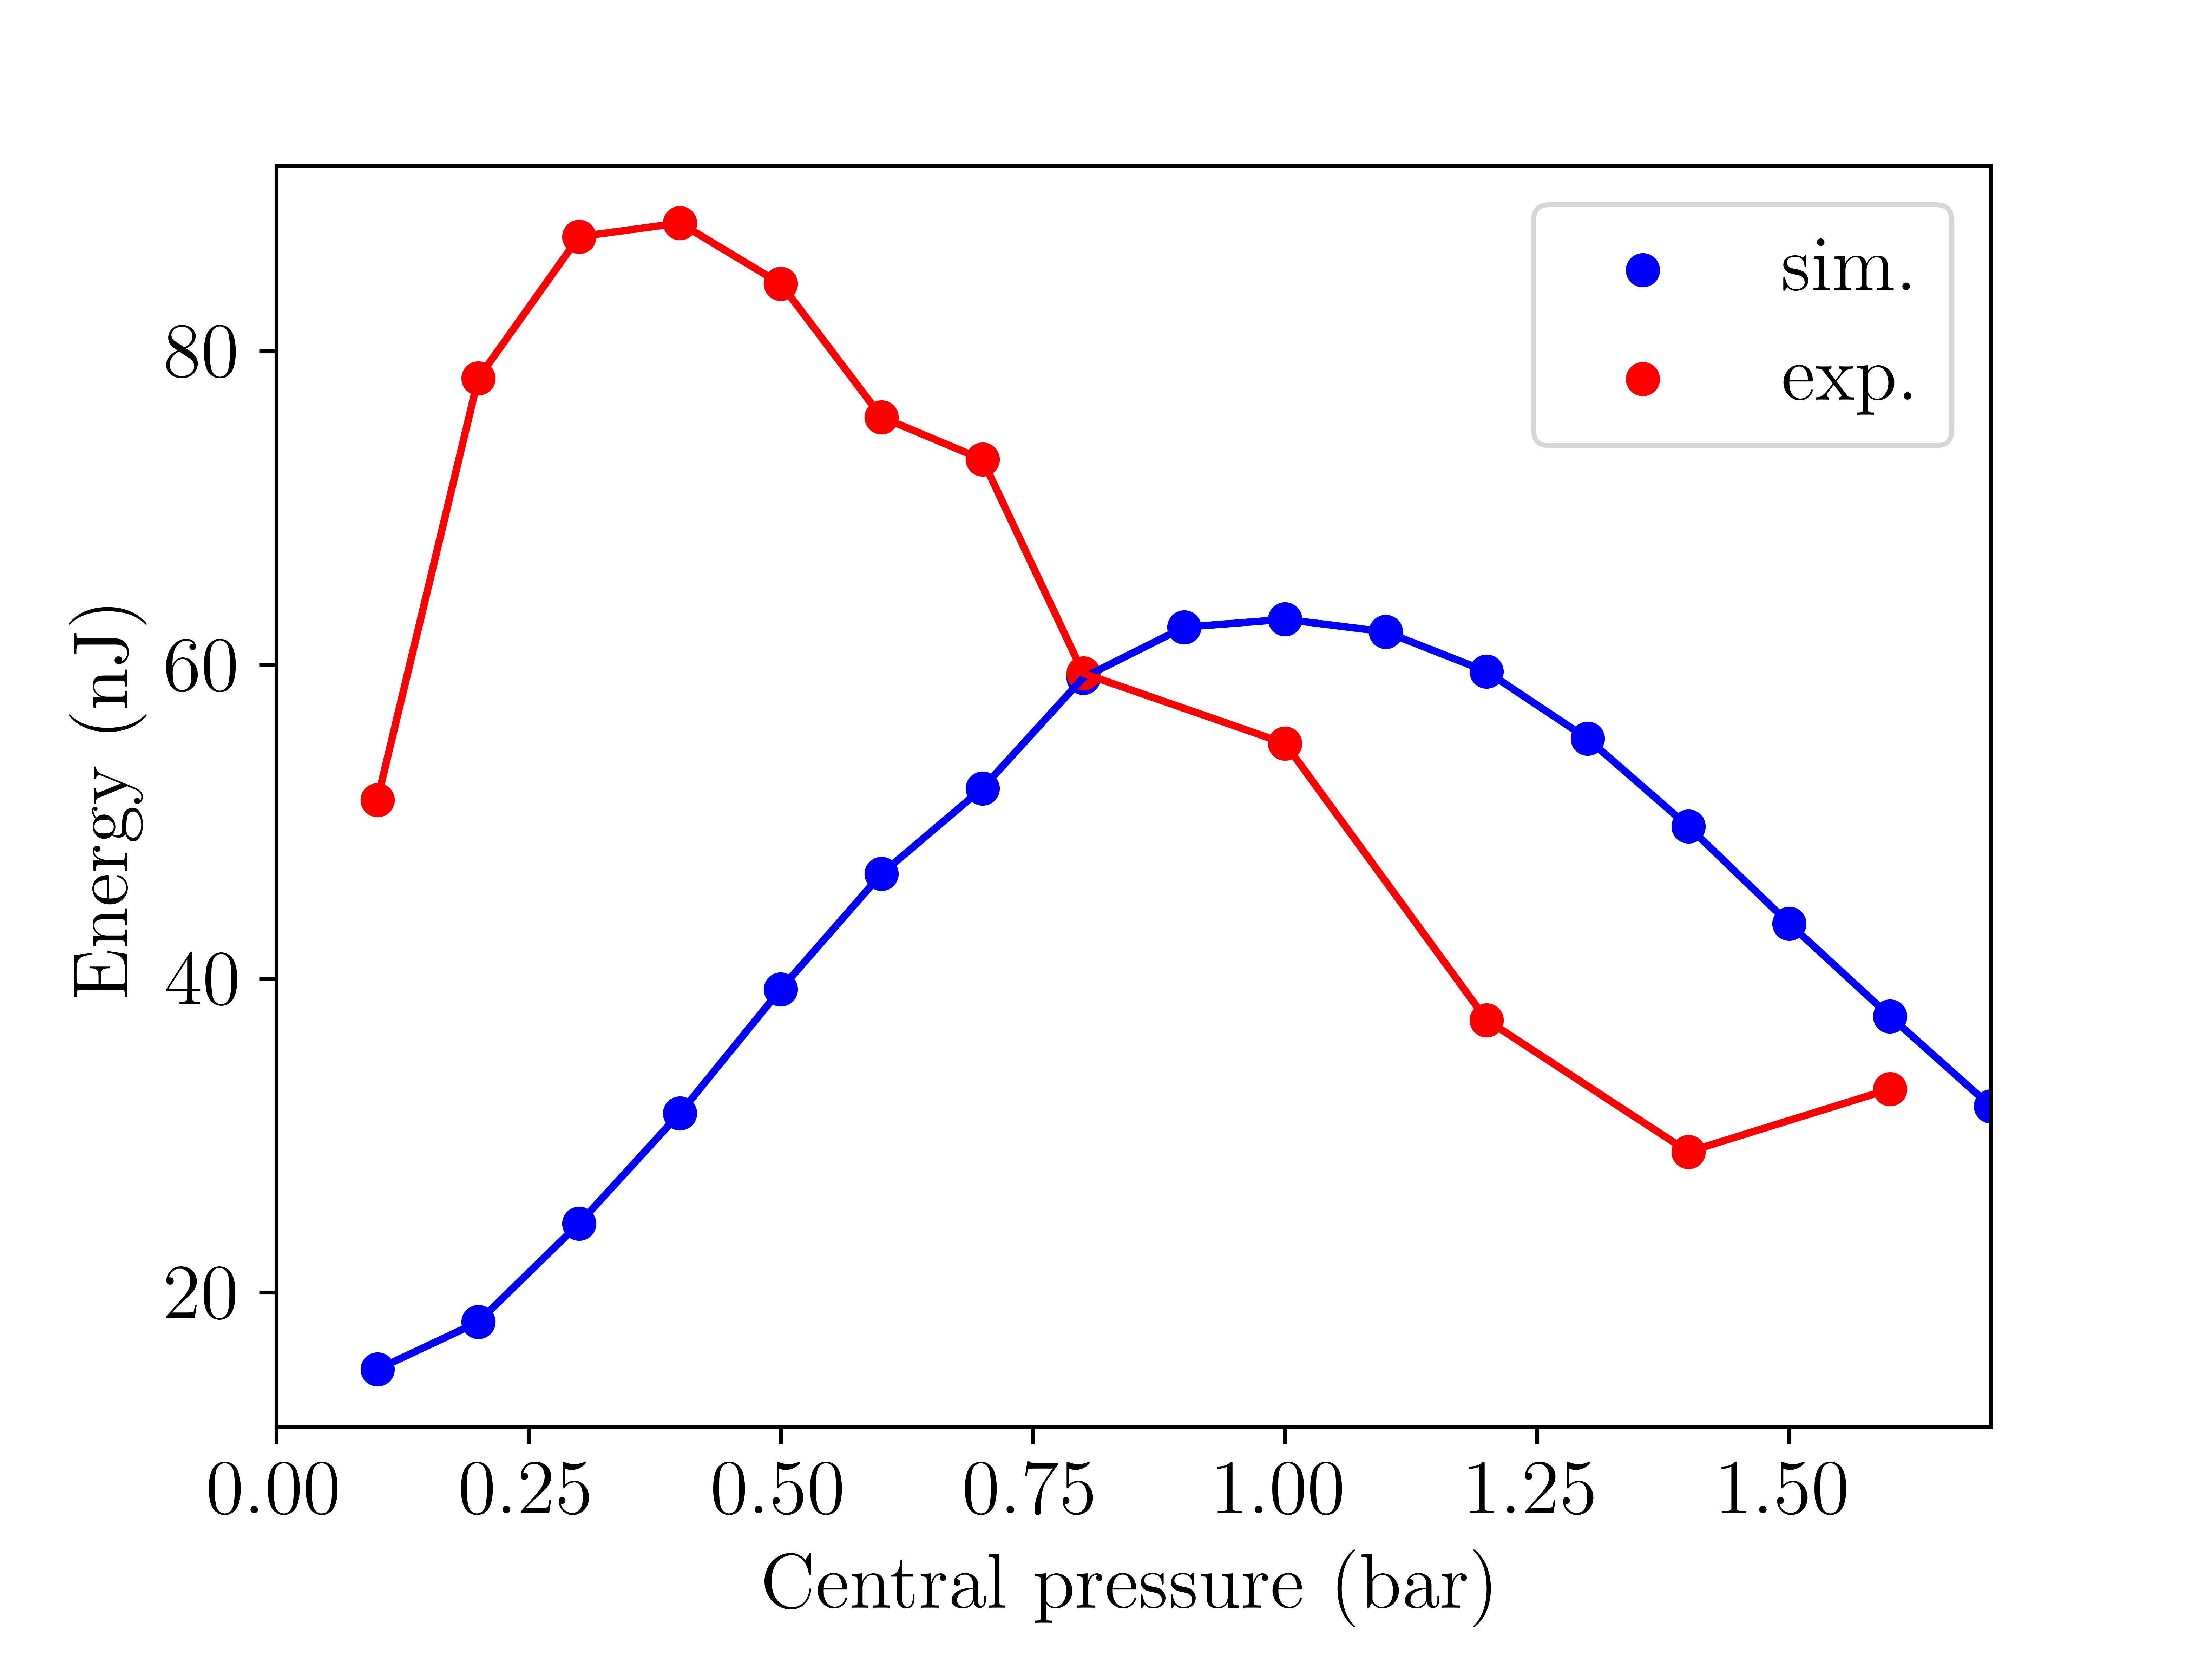
\includegraphics[scale=0.5]{im/energies}\label{im:pressure_scan}
\caption{Argon pressure scan at 150mW input beam power.}
\end{figure}
\end{center}

\textcolor{red}{test image}
\begin{center}
\begin{figure}[h]
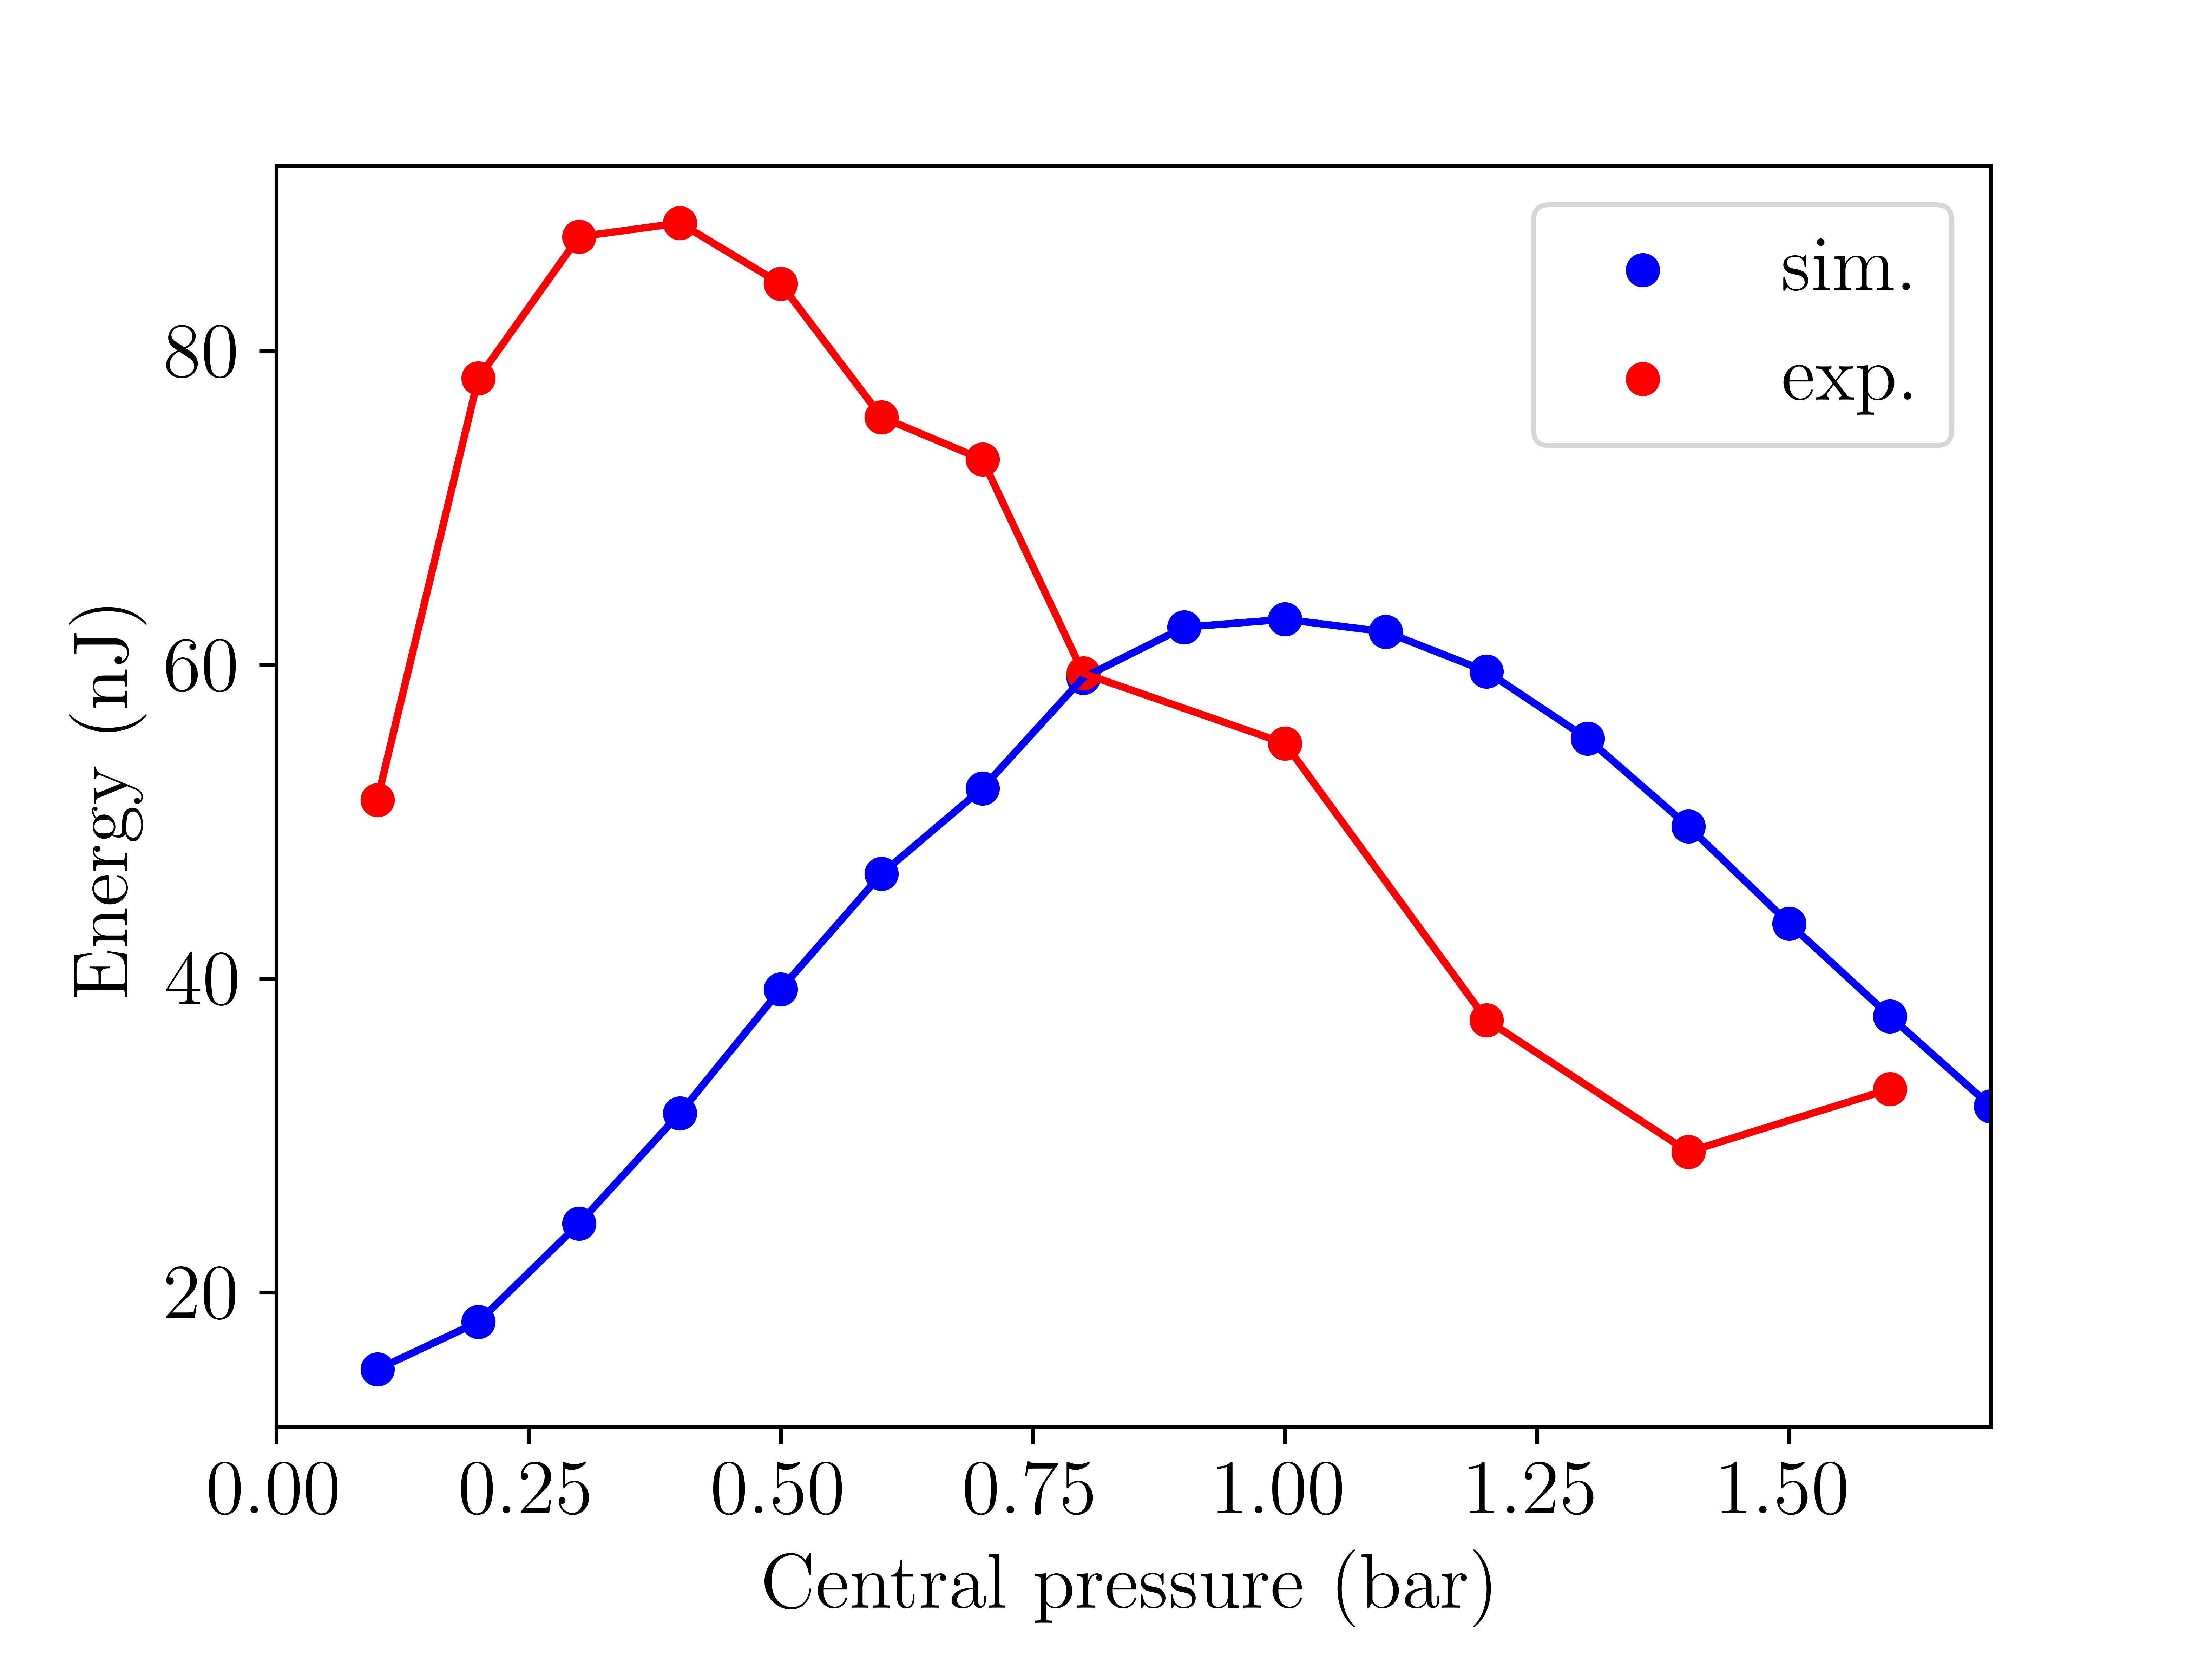
\includegraphics[scale=0.5]{im/energies}\label{im:pressure_scan}
\caption{Argon pressure scan at 150mW input beam power.}
\end{figure}
\end{center}

\cite{reiter2010}

\section{Discussion}

\textcolor{red}{
Comparison with results at times difficult: pressure and energy of output beam hard to measure, same for pulse duration}

\textcolor{red}{
Many more factors to be investigated (beam focus position, beam size, higher beam powers...)}

\textcolor{red}{
Take into account beam spatial profile (astigmatism, deformation,...) [although that requires moving away from a Hankel transform and breaking radialt symmetry]
}
\textcolor{red}{
Improve simulations by improving COMSOL gas density model (need to use high Mach number model instead, current model does not take into account gas interaction). 
}

\section{Conclusions}
\textcolor{red}{summarise everything}


\section*{Acknowledgments}
\textcolor{red}{I want to thank Josina Hahne for the supervision of the project and all of her support, as well as Vincent Wanie for his additional guidance. I also want to thank Chris Brahms for providing help with \textit{Luna.jl} as well as Olaf Behnke and Andreas Przystawik for organising the DESY Summer Student programme.}  


\section*{References}
\bibliographystyle{osa}
\bibliography{refs.bib}

\end{document}